\chapter{إحصاء القياس الكيميائي}\label{ch:b2:measurement-statistics}

يقيس مختبران الرصاص في ماء الصنبور نفسه ويعلنان 9.6 و\qty{11.2}{\micro g/L}.
والقيمة الإرشادية لمياه الشرب \qty{10}{\micro g/L}. فهل الماء صالح للشرب؟ وهل يختلف
المختبران حقًا، أم أن النتيجتين هما القيمة نفسها مرئية عبر تشتت
قياسين؟ إن الرقم الناتج من تحليل لا يعني شيئًا دون ارتيابه، ويقدم هذا الفصل
أدوات حسابه: إحصاء القياسات المتكررة، وانتشار الارتياب
عبر حساب، والمعايرة بالمربعات الصغرى، والحدود التي لا ترى الطريقة شيئًا تحتها.
% ledger: who:lead

\begin{omfigure}
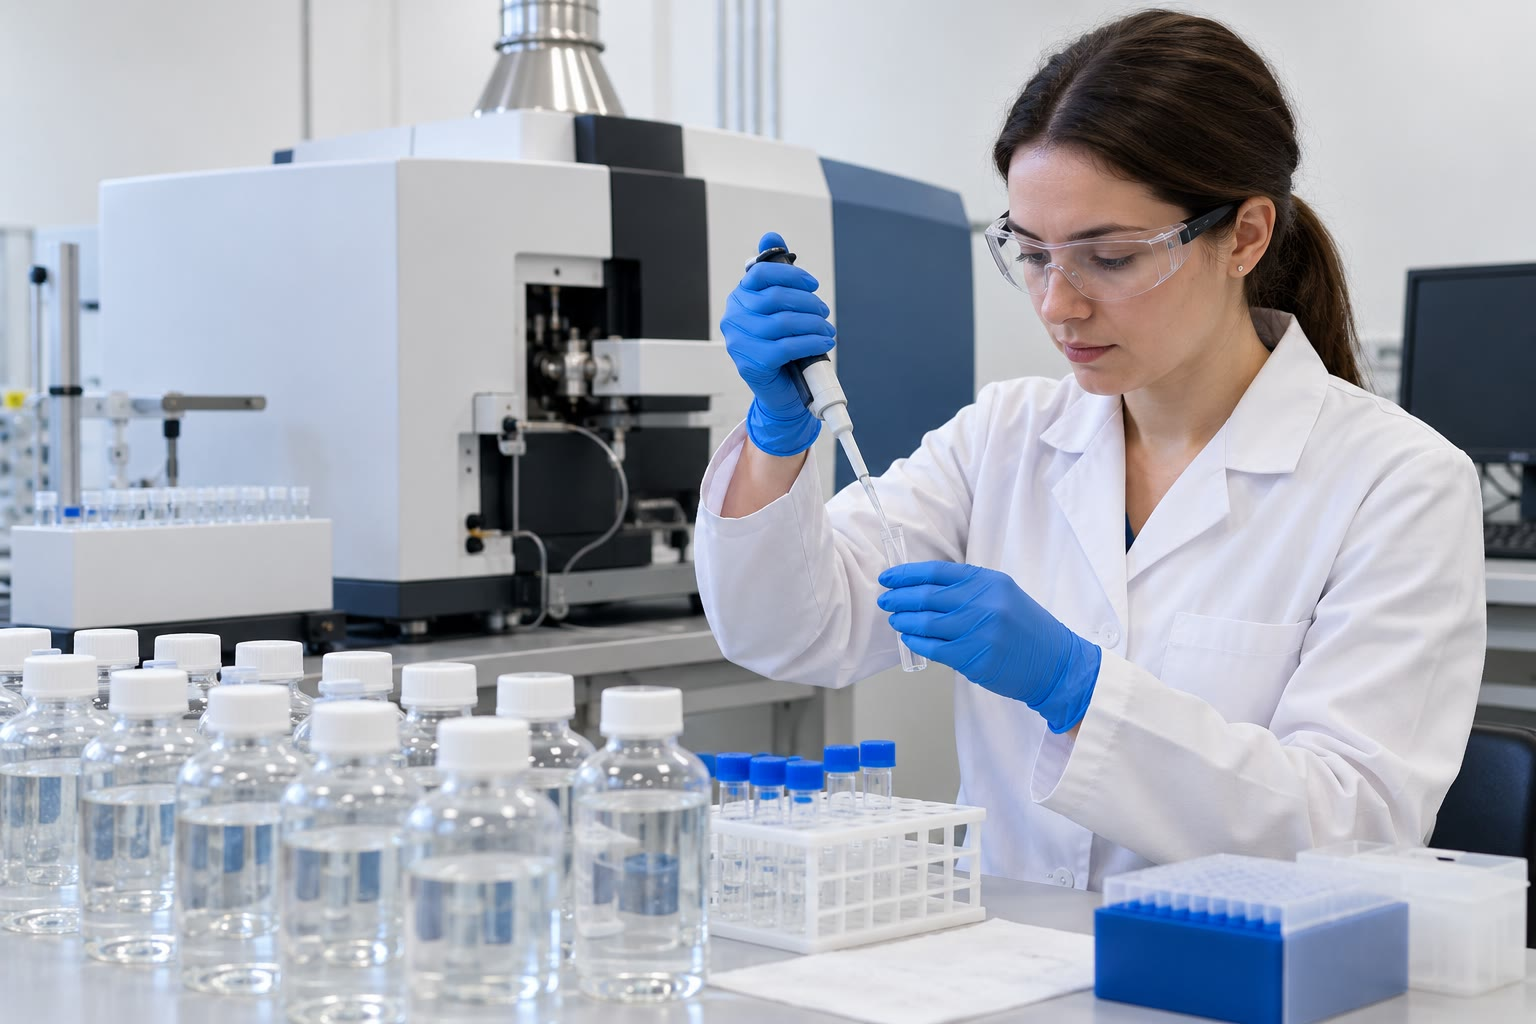
\includegraphics[width=0.56\linewidth]{images/book3/ai/b2-34-water-lab.jpg}

{\small مختبر لفحص المياه: قوارير عينات، وتقني يسحب بالماصة، ومحلل عنصري
في الخلف (رسم توضيحي).}
\end{omfigure}

\begin{recall}
مجلد السنة الأولى: ارتياب القياس، والارتياب المعياري، والتقييمان من النوع A والنوع B،
والارتياب الموسع، والارتياب النسبي، والانحراف المنظَّم $z$ بين قيمتين، 
والوعد ببرهان $u(\bar x) = s/\sqrt n$ وبقاعدة انتشار عامة. والمجلد المدرسي:
\omterm{def:b2:measurement-statistics:calibration}{مستقيم المعايرة}. و\cref{ch:b2:mass-spec-atomic}: الامتصاص الذري.
\end{recall}

\section{القياسات المتكررة}

كرّر قياسًا تتشتت النتائج. ونعامل كل نتيجة $x_i$ بوصفها متغيرًا عشوائيًا
متوسطه $\mu$ (القيمة التي تعطيها الطريقة في المتوسط) وانحرافه المعياري $\sigma$؛ وحين تتجمع أسباب
كثيرة صغيرة مستقلة، تتبع النتائج القانون الطبيعي (الغاوسي)، فيقع نحو 68~\% منها
ضمن $\mu \pm \sigma$ و95~\% ضمن $\mu \pm 1.96\sigma$.

\begin{definition}[التشتت]\label{def:b2:measurement-statistics:dispersion}
من أجل $n$ نتيجة $x_1, \dots, x_n$ متوسطها $\bar x$، يكون \emph{الانحراف المعياري
التجريبي}\index{انحراف معياري تجريبي} هو $s = \sqrt{\sum (x_i - \bar x)^2/(n-1)}$؛ وهو
يقدّر $\sigma$. و\emph{الانحراف المعياري للمتوسط}\index{انحراف معياري للمتوسط} هو
الانحراف المعياري للمتوسط $\bar x$ على سلاسل كثيرة من $n$ نتيجة، ومقداره التقديري $s/\sqrt n$.
\end{definition}

يصحح المقسوم عليه $n - 1$ بدلًا من $n$ كون الانحرافات مأخوذة عن $\bar x$،
المحسوب هو نفسه من المعطيات ذاتها، مما يجعلها أصغر قليلًا مما ينبغي: والمقدار $n - 1$ هو عدد
الانحرافات المستقلة، أي درجات الحرية.

\begin{theorem}[تباين المتوسط]\label{thm:b2:measurement-statistics:mean-variance}
إذا كانت $x_1, \dots, x_n$ مستقلة، تباين كل منها $\sigma^2$، فإن $\operatorname{var}(\bar x) =
\sigma^2/n$: \omterm{def:b2:measurement-statistics:dispersion}{فالانحراف المعياري للمتوسط} هو $\sigma/\sqrt n$.
\end{theorem}

\begin{proof}
من أجل متغيرات مستقلة يكون تباين المجموع مجموع التباينات، 
و$\operatorname{var}(cX) = c^2\operatorname{var}(X)$. إذن $\operatorname{var}(\bar x) =
\operatorname{var}\bigl(\tfrac1n\sum x_i\bigr) = \tfrac{1}{n^2}\sum\operatorname{var}(x_i) =
\tfrac{1}{n^2}\,n\sigma^2 = \sigma^2/n$. وتعويض $\sigma$ بتقديرها $s$ يعطي الارتياب المعياري
من النوع A $u(\bar x) = s/\sqrt n$ المقبول في مجلد السنة الأولى.
\end{proof}

\section{مجالات الثقة}

\begin{definition}[مجال الثقة]\label{def:b2:measurement-statistics:confidence}
\emph{مجال الثقة}\index{مجال الثقة} عند \emph{مستوى الثقة}\index{مستوى الثقة}
$1 - \alpha$ (95~\% غالبًا) مجال يُحسب من المعطيات بقاعدة إذا طُبقت على
سلاسل كثيرة احتوى القيمة الحقيقية في كسر $1 - \alpha$ منها. ومن أجل متوسط $n$ نتيجة يكون
$\bar x \pm t\,s/\sqrt n$، حيث $t$ هو \emph{معامل ستيودنت}\index{معامل ستيودنت}
من أجل $n - 1$ درجة حرية وذلك المستوى.
\end{definition}

\begin{proposition}[قانون ستيودنت]\label{prop:b2:measurement-statistics:student}
من أجل $n$ نتيجة طبيعية مستقلة، يتبع $T = (\bar x - \mu)/(s/\sqrt n)$ قانون ستيودنت ذا
$n - 1$ درجة حرية، الذي كثافته متناسبة مع $(1 + t^2/\nu)^{-(\nu+1)/2}$ مع
$\nu = n - 1$. وهو أعرض من القانون الطبيعي ويؤول إليه كلما كبرت $n$.
\end{proposition}

\admitted

القسمة على $s$ بدلًا من $\sigma$ المجهولة تضيف تشتت $s$ نفسها، وهو كبير حين تكون $n$
صغيرة؛ ومن هنا الذيول الأثقل، والمعاملات الأكبر من 1.96. ويعطي الجدول معاملات 95~\%،
المحسوبة من الكثافة.

\begin{omfigure}
\begin{minipage}[c]{0.56\linewidth}
\begin{tikzpicture}
\begin{axis}[width=\linewidth, height=4.8cm, xmin=-5, xmax=5, ymin=0, ymax=0.43,
  xlabel={$t$}, ylabel={الكثافة}, label style={font=\small}, tick label style={font=\scriptsize},
  legend style={font=\scriptsize, at={(0.98,0.98)}, anchor=north east}, legend cell align=left]
\addplot[omThm, thick] table[x=t, y=nu2] {figdata/out/bachelor-2-regression-c.dat};
\addplot[omMeth, thick] table[x=t, y=nu5] {figdata/out/bachelor-2-regression-c.dat};
\addplot[black, thick, dashed] table[x=t, y=normal] {figdata/out/bachelor-2-regression-c.dat};
\legend{$\nu = 2$, $\nu = 5$, طبيعي}
\end{axis}
\end{tikzpicture}
\end{minipage}\hfill
\begin{minipage}[c]{0.4\linewidth}\centering
\small
\begin{tabular}{rr}
\hline
$\nu = n - 1$ & $t$ (95~\%) \\
\hline
1 & 12.706 \\
2 & 4.303 \\
3 & 3.182 \\
4 & 2.776 \\
5 & 2.571 \\
9 & 2.262 \\
20 & 2.086 \\
$\infty$ & 1.960 \\
\hline
\end{tabular}
\end{minipage}
\par\vspace{4pt}

{\small كثافتا ستيودنت لدرجتي حرية 2 و5 مقابل القانون الطبيعي، ومعاملات 95~\%
الثنائية الطرف، المحسوبة بمكاملة الكثافة (والسطر الأخير هو القانون الطبيعي).}
% figdata: bachelor-2/regression.py parts c, e
\end{omfigure}

\begin{method}[مجال ثقة لمتوسط]\label{met:b2:measurement-statistics:confidence-interval}
\begin{enumerate}
  \item احسب $\bar x$ و$s$ للنتائج البالغ عددها $n$؛ وتحقق من أن لا نتيجة شاذة شذوذًا فاحشًا.
  \item اقرأ $t$ من أجل $\nu = n - 1$ عند المستوى المختار.
  \item أعلن $\bar x \pm t\,s/\sqrt n$، مع تقريب الارتياب إلى رقم معنوي أو رقمين
        وتقريب المتوسط إلى المنزلة العشرية نفسها.
  \item للمقارنة بقيمة مرجعية $x_{\mathrm{ref}}$، احسب $|\bar x - x_{\mathrm{ref}}|/(s/\sqrt
        n)$: فإن تجاوزت $t$، كان الفرق معنويًا عند ذلك المستوى؛ وإلا، فالمعطيات لا تُظهر
        فرقًا (وهذا لا يثبت أنه غير موجود).
\end{enumerate}
\end{method}

\section{انتشار الارتياب}

\begin{theorem}[قانون انتشار الارتياب]\label{thm:b2:measurement-statistics:propagation}
إذا كانت $y = f(x_1, \dots, x_n)$، حيث $x_i$ مستقلة وارتياباتها المعيارية $u(x_i)$ صغيرة
بما يكفي لتكون $f$ خطية تقريبًا عليها، فإن
\begin{equation*}
u^2(y) = \sum_{i=1}^{n}\left(\frac{\partial f}{\partial x_i}\right)^2 u^2(x_i).
\end{equation*}
\end{theorem}

\begin{proof}
حتى الرتبة الأولى (تايلور)، $y - f(\mu_1, \dots, \mu_n) \approx \sum c_i(x_i - \mu_i)$ مع $c_i = \partial
f/\partial x_i$ عند المتوسطات. وتباين التركيب الخطي لمتغيرات مستقلة هو
$\sum c_i^2\operatorname{var}(x_i)$ (كما في \cref{thm:b2:measurement-statistics:mean-variance})؛ ومع
$\operatorname{var}(x_i) = u^2(x_i)$ نحصل على النتيجة.
\end{proof}

\begin{corollary}[المجاميع والجداءات]\label{cor:b2:measurement-statistics:products}
في المجموع أو الفرق، تُجمع الارتيابات المعيارية تربيعيًا: $u^2(x_1 \pm x_2) = u^2(x_1) +
u^2(x_2)$. وفي الجداء أو الحاصل $y = x_1^{a}x_2^{b}\cdots$، تُجمع الارتيابات النسبية
تربيعيًا، كل منها موزون بأسّه: $\bigl(u(y)/y\bigr)^2 = a^2\bigl(u(x_1)/x_1\bigr)^2 +
b^2\bigl(u(x_2)/x_2\bigr)^2 + \cdots$
\end{corollary}

\begin{proof}
في المجموع المشتقات الجزئية $\pm1$. ومن أجل $y = x_1^ax_2^b$، $\partial y/\partial x_1 =
a\,y/x_1$ و$\partial y/\partial x_2 = b\,y/x_2$؛ فتعطي المبرهنة $u^2(y) = a^2y^2u^2(x_1)/x_1^2 +
b^2y^2u^2(x_2)/x_2^2$؛ ثم نقسم على $y^2$.
\end{proof}

\begin{method}[إجراء الانتشار]\label{met:b2:measurement-statistics:propagate}
\begin{enumerate}
  \item اكتب النتيجة صيغةً بدلالة المقادير المقيسة؛ وعدّد كل مُدخل مع ارتيابه
        المعياري (من النوع A أو B).
  \item في الجداءات والحواصل، اعمل بالارتيابات النسبية؛ وفي المجاميع، بالمطلقة؛
        وإلا فخذ المشتقات الجزئية.
  \item اجمع تربيعيًا؛ وأوجد الحد الغالب: فتحسين الحدود الأخرى جهد ضائع.
  \item اضرب في عامل التغطية (2، أو $t$ ستيودنت حين يأتي الحد الغالب من تكرارات
        قليلة) للحصول على ارتياب موسع.
\end{enumerate}
\end{method}

\section{المعايرة}

\begin{definition}[منحنى المعايرة]\label{def:b2:measurement-statistics:calibration}
\emph{منحنى المعايرة}\index{منحنى المعايرة} يربط إشارة جهاز $y$ بالتركيز
$x$، انطلاقًا من معايير معلومة التركيز. و\emph{مستقيم المربعات
الصغرى}\index{مستقيم المربعات الصغرى} $y = a + bx$ هو المستقيم الذي يجعل $S = \sum (y_i - a -
bx_i)^2$ أصغر ما يمكن؛ وكل $e_i = y_i - a - bx_i$ هو \emph{باقٍ}\index{باق}.
\end{definition}

\begin{theorem}[مستقيم المربعات الصغرى]\label{thm:b2:measurement-statistics:least-squares}
مع المتوسطين $\bar x$، $\bar y$، و$S_{xx} = \sum(x_i - \bar x)^2$ و$S_{xy} = \sum(x_i - \bar x)(y_i -
\bar y)$، يكون \omterm{def:b2:measurement-statistics:calibration}{لمستقيم المربعات الصغرى}
\begin{equation*}
b = \frac{S_{xy}}{S_{xx}}, \qquad a = \bar y - b\bar x.
\end{equation*}
\end{theorem}

\begin{proof}
$S$ دالة تربيعية في $a$ و$b$. وتنعدم مشتقاتها الجزئية عند القيمة الصغرى:
$\partial S/\partial a = -2\sum(y_i - a - bx_i) = 0$ يعطي $a = \bar y - b\bar x$؛ وبالتعويض في
$\partial S/\partial b = -2\sum x_i(y_i - a - bx_i) = 0$ نحصل على $\sum x_i\bigl((y_i - \bar y) - b(x_i -
\bar x)\bigr) = 0$، أي $S_{xy} = bS_{xx}$ (لأن $\sum \bar x(y_i - \bar y) = \sum \bar x(x_i - \bar
x) = 0$). والمشتقات الثانية تكوّن المصفوفة
\[\begin{pmatrix} 2n & 2\sum x_i\\ 2\sum x_i & 2\sum x_i^2\end{pmatrix},\]
التي قطرها موجب ومحددها $4nS_{xx}$ موجب حين لا تكون $x_i$ كلها
متساوية: فالنقطة المستقرة قيمة صغرى.
\end{proof}

\begin{proposition}[قراءة تركيز]\label{prop:b2:measurement-statistics:interpolation}
من أجل $n$ معيارًا انحرافها المعياري الباقي $s_{y/x} = \sqrt{\sum e_i^2/(n-2)}$، فإن عينة تُقرأ
$m$ مرة بمتوسط إشارة $\bar y_0$ لها $x_0 = (\bar y_0 - a)/b$ وانحراف معياري
\begin{equation*}
s_{x_0} = \frac{s_{y/x}}{b}\sqrt{\frac1m + \frac1n + \frac{(\bar y_0 - \bar y)^2}{b^2S_{xx}}},
\end{equation*}
يُستعمل مع $t$ ستيودنت من أجل $n - 2$ درجة حرية.
\end{proposition}

\admitted

الحدود الثلاثة تحت الجذر هي تشتت قراءات العينة، وارتياب ارتفاع المستقيم
وارتياب ميله؛ والأخير ينعدم عند مركز مجال المعايرة، وهو حيث
تُقرأ العينات على أفضل وجه.

\begin{omfigure}
\begin{tikzpicture}
\begin{axis}[width=0.5\linewidth, height=5cm, xmin=-1, xmax=22, ymin=0, ymax=0.22,
  xlabel={\foreignlanguage{arabic}{الرصاص \babelsublr{(\unit{\micro g/L})}}}, ylabel={الامتصاصية}, label style={font=\small},
  tick label style={font=\scriptsize}, scaled y ticks=false,
  yticklabel style={/pgf/number format/fixed, /pgf/number format/precision=2}]
\addplot[omDef, thick] table[x=x, y=line] {figdata/out/bachelor-2-regression-b.dat};
\addplot[only marks, mark=*, mark size=1.8pt, omThm] table[x=x, y=A] {figdata/out/bachelor-2-regression-a.dat};
\end{axis}
\end{tikzpicture}\hfill
\begin{tikzpicture}
\begin{axis}[width=0.5\linewidth, height=5cm, xmin=-1, xmax=22, ymin=-0.002, ymax=0.002,
  xlabel={\foreignlanguage{arabic}{الرصاص \babelsublr{(\unit{\micro g/L})}}}, ylabel={الباقي}, label style={font=\small},
  tick label style={font=\scriptsize}, scaled y ticks=false, ycomb,
  yticklabel style={/pgf/number format/fixed, /pgf/number format/precision=3},
  extra y ticks={0}, extra y tick style={grid=major, grid style={black!50}}]
\addplot[omThm, thick, mark=*, mark size=1.6pt] table[x=x, y=res] {figdata/out/bachelor-2-regression-a.dat};
\end{axis}
\end{tikzpicture}

{\small معايرة الرصاص بالامتصاص الذري في الفرن الغرافيتي عند \qty{283.3}{nm} (معطيات تمرين،
مستعملة في المسألة). يمينًا: المعايير الخمسة \omterm{def:b2:measurement-statistics:calibration}{ومستقيم المربعات الصغرى}. يسارًا: \omterm{def:b2:measurement-statistics:calibration}{البواقي}، صغيرة
وبلا نمط: فالمستقيم كافٍ.}
% figdata: bachelor-2/regression.py parts a, b
% ledger: asd:Pb283
\end{omfigure}

\begin{method}[إجراء المعايرة]\label{met:b2:measurement-statistics:calibrate}
\begin{enumerate}
  \item حضّر خمسة معايير أو أكثر تغطي المجال المتوقع، في المصفوفة نفسها التي في العينات،
        ومحلولًا شاهدًا.
  \item طابق \omterm{def:b2:measurement-statistics:calibration}{مستقيم المربعات الصغرى}؛ وارسم \omterm{def:b2:measurement-statistics:calibration}{البواقي}. فالنمط المنحني يعني أن الاستجابة غير
        خطية: ضيّق المجال أو طابق منحنى. والباقي الكبير الوحيد يشير إلى معيار معيب.
  \item اقرأ العينات، ويُفضَّل قرب منتصف المجال، بتكرار؛ واحسب $x_0$ 
        و$s_{x_0}$.
  \item أعلن $x_0 \pm t\,s_{x_0}$ بعد التصحيح لكل تخفيف، مع إضافة الارتياب المنتشر
        للتخفيف إن لم يكن مهملًا.
\end{enumerate}
\end{method}

\begin{definition}[الإضافة القياسية]\label{def:b2:measurement-statistics:standard-addition}
في \emph{طريقة الإضافة القياسية}\index{طريقة الإضافة القياسية}، تُضاف كميات معلومة من المادة المحللة
إلى أجزاء متساوية من العينة نفسها؛ وتُرسم الإشارة بدلالة التركيز المضاف،
ويكون تركيز المادة المحللة في العينة هو المسافة من المبدأ إلى النقطة التي يقطع فيها
المستقيم الممدود حتى الإشارة المعدومة المحور، أي $a/b$.
\end{definition}

\begin{method}[الإضافة القياسية]\label{met:b2:measurement-statistics:standard-addition}
\begin{enumerate}
  \item استعملها حين تغيّر مصفوفة العينة الاستجابة (الأملاح، والأحماض، والمادة العضوية)، بحيث
        تعطي المعايير المحضرة في الماء النقي ميلًا خطأ.
  \item أضف إلى أجزاء متساوية كميات معلومة متزايدة، وخفف الكل إلى الحجم نفسه، ثم قِس.
  \item طابق المستقيم؛ فيكون التركيز في المحاليل المقيسة $a/b$؛ وصحّح للتخفيف.
  \item يجب أن تكون الاستجابة خطية انطلاقًا من الصفر: تحقق من \omterm{def:b2:measurement-statistics:calibration}{البواقي}.
\end{enumerate}
\end{method}

\begin{omfigure}
\begin{tikzpicture}
\begin{axis}[width=0.62\linewidth, height=5cm, xmin=-4, xmax=7, ymin=0, ymax=0.42,
  xlabel={\foreignlanguage{arabic}{التركيز المضاف \babelsublr{(\unit{mg/L})}}}, ylabel={الامتصاصية}, label style={font=\small},
  tick label style={font=\scriptsize}, axis lines=left, scaled y ticks=false,
  yticklabel style={/pgf/number format/fixed, /pgf/number format/precision=1}]
\draw[black!40] (axis cs:0,0) -- (axis cs:0,0.42);
\addplot[omDef, thick, densely dashed] table[x=x, y=line] {figdata/out/bachelor-2-regression-d-line.dat};
\addplot[only marks, mark=*, mark size=1.8pt, omThm] table[x=x, y=A] {figdata/out/bachelor-2-regression-d.dat};
\draw[<->, omMeth, thick] (axis cs:-3.11,0.06) -- (axis cs:0,0.06); \node[omMeth, below, font=\scriptsize] at (axis cs:-0.8,0.055) {$a/b$};
\end{axis}
\end{tikzpicture}

{\small الإضافة القياسية (معطيات تمرين): امتصاصية عينة أُضيف إليها 0 و2 و4 
و\qty{6}{mg/L} من المادة المحللة. يلاقي المستقيم الإشارة المعدومة عند \qty{-3.11}{mg/L}: فالمحلول المقيس
كان يحوي \qty{3.11}{mg/L}.}
% figdata: bachelor-2/regression.py part d
\end{omfigure}

\section{الكشف والتقدير الكمي والمصادقة}

\begin{definition}[الحدود]\label{def:b2:measurement-statistics:limits}
\emph{حد الكشف}\index{حد الكشف} لطريقة هو أصغر تركيز يمكن تمييز إشارته
من إشارة الشاهد بخطر صغير معلن لكشف كاذب؛ 
و\emph{حد التقدير الكمي}\index{حد التقدير الكمي} هو أصغر تركيز يمكن
قياسه بارتياب نسبي مقبول.
\end{definition}

\begin{proposition}[تقديرات شائعة]\label{prop:b2:measurement-statistics:lod}
مع $s_{\mathrm{blank}}$ الانحراف المعياري لإشارات الشاهد المتكررة و$b$ ميل
\omterm{def:b2:measurement-statistics:calibration}{مستقيم المعايرة}، $x_{\mathrm{LOD}} \approx 3s_{\mathrm{blank}}/b$ و$x_{\mathrm{LOQ}} \approx
10s_{\mathrm{blank}}/b$.
\end{proposition}

\begin{proof}[تعليل]
إذا كانت إشارات الشاهد طبيعية بانحراف معياري $s_{\mathrm{blank}}$، فإن الشاهد يتجاوز متوسطه
بأكثر من $3s_{\mathrm{blank}}$ باحتمال نحو 0.13~\% (الذيل الأحادي الجانب للقانون الطبيعي بعد
3 انحرافات معيارية): فوصف الإشارة بأنها «مكشوفة» فوق تلك العتبة نادرًا ما يخلط شاهدًا
بعينة. والإشارة التي تزيد على الشاهد بمقدار $10s_{\mathrm{blank}}$ لها انحراف معياري نسبي نحو
10~\%، وهي العتبة المعتادة لنتيجة كمية. والقسمة على $b$ تحوّل الإشارات إلى
تراكيز.
\end{proof}

\begin{definition}[المصادقة]\label{def:b2:measurement-statistics:validation}
\emph{الصحة}\index{صحة} هي قرب متوسط عدد كبير من النتائج من القيمة
الحقيقية؛ والفرق بينهما هو \emph{الانحياز}\index{انحياز}. و\emph{الإحكام}\index{إحكام} هو
قرب النتائج المستقلة بعضها من بعض، معبَّرًا عنه بانحراف معياري:
\emph{قابلية التكرار}\index{قابلية التكرار} في الظروف نفسها (المشغّل نفسه، والجهاز،
والمختبر، وزمن قصير)، و\emph{قابلية الاستنساخ}\index{قابلية الاستنساخ} في ظروف متغيرة
(مختبرات مختلفة). و\emph{المصادقة على الطريقة}\index{مصادقة على الطريقة} هي مجموعة التجارب
التي تثبت، لطريقة ما، صحتها، وإحكامها، وخطيتها ومجالها، وحدي كشفها
وتقديرها الكمي.
\end{definition}

يُتحقق من \omterm{def:b2:measurement-statistics:validation}{الصحة} بمادة مرجعية معتمدة أو بالإضافة؛ ومن \omterm{def:b2:measurement-statistics:validation}{الإحكام} بالتكرارات في
مختبر واحد وبالمقارنات بين المختبرات. وقد تكون الطريقة محكمة لكنها منحازة، كل
نتيجة قريبة من الأخرى وكلها خطأ: \omterm{def:b2:measurement-statistics:validation}{فالإحكام} ليس برهانًا على \omterm{def:b2:measurement-statistics:validation}{الصحة}.

\begin{history}[ستيودنت، 1908]
\begin{minipage}[t]{0.17\linewidth}
\vspace{0pt}
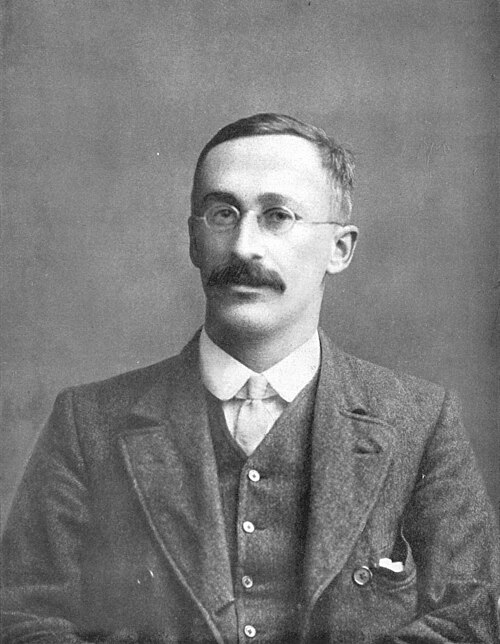
\includegraphics[width=\linewidth]{images/book3/gosset.jpg}
\end{minipage}\hfill
\begin{minipage}[t]{0.79\linewidth}
\vspace{0pt}
كان على وليام سيلي غوسيت، الكيميائي العامل لدى مصنع جعة، أن يحكم على المواد الخام انطلاقًا من عينات قليلة جدًا،
أقل بكثير مما يلزم للقانون الطبيعي. وفي سنة 1908 نشر توزيع المتوسط مقسومًا على الانحراف المعياري
للعينة، تحت الاسم المستعار «ستيودنت» لأن مشغّله لم يكن يسمح للموظفين بالنشر
بأسمائهم. ويُستعمل قانون ستيودنت كلما أعلن محلل مجالًا انطلاقًا من ثلاث أو أربع
تكرارات. (صورة، 1908: ملكية عامة؛ ويكيميديا كومنز.)
\end{minipage}
\end{history}

\section{تمارين}

\begin{exercise}[$\star$]\label{exo:b2:measurement-statistics:1}
تعطي خمس معايرات 12.45 و12.50 و12.48 و12.52 و\qty{12.46}{mL}. احسب المتوسط، 
\omterm{def:b2:measurement-statistics:dispersion}{والانحراف المعياري التجريبي} \omterm{def:b2:measurement-statistics:dispersion}{والانحراف المعياري للمتوسط}.
\end{exercise}

\begin{exercise}[$\star$]\label{exo:b2:measurement-statistics:2}
أعطِ \omterm{def:b2:measurement-statistics:confidence}{مجال الثقة} 95~\% لمتوسط التمرين~1.
\end{exercise}

\begin{exercise}[$\star$]\label{exo:b2:measurement-statistics:3}
يُحضَّر محلول بإذابة $m = \qty{0.5000}{g}$ ($u = \qty{0.0002}{g}$) من صلب في دورق
$V = \qty{250.0}{mL}$ ($u = \qty{0.15}{mL}$). احسب الارتياب المعياري النسبي للمقدار $c = m/(MV)$،
والكتلة المولية دقيقة بما يكفي.
\end{exercise}

\begin{exercise}[$\star$]\label{exo:b2:measurement-statistics:4}
طابق \omterm{def:b2:measurement-statistics:calibration}{مستقيم المربعات الصغرى} المار بالنقاط $(0, 0.02)$، $(1, 0.21)$، $(2, 0.39)$، $(3, 0.62)$.
\end{exercise}

\begin{exercise}[$\star\star$]\label{exo:b2:measurement-statistics:5}
محلول مرجعي معتمد يحوي \qty{10.00}{mg/L} من عنصر. وتعطي خمسة تحاليل متوسطًا قدره
\qty{10.12}{mg/L} مع $s = \qty{0.08}{mg/L}$. هل الطريقة منحازة عند المستوى 95~\%؟
\end{exercise}

\begin{exercise}[$\star\star$]\label{exo:b2:measurement-statistics:6}
تركيز أيونات الهيدرونيوم معلوم بارتياب معياري نسبي قدره 2~\%. ما
الارتياب المعياري للأس الهيدروجيني pH؟
\end{exercise}

\begin{exercise}[$\star\star$]\label{exo:b2:measurement-statistics:7}
لعشرة شواهد $s = 0.0012$ وحدة امتصاصية؛ وميل المعايرة \qty{0.0098}{L/\micro g}.
قدّر حدي الكشف والتقدير الكمي.
\end{exercise}

\begin{exercise}[$\star\star$]\label{exo:b2:measurement-statistics:8}
في تجربة الإضافة القياسية في الشكل، كانت الأجزاء الأربعة محضَّرة بتخفيف
\qty{10.0}{mL} من العينة إلى \qty{50.0}{mL}. أعطِ التركيز في العينة.
\end{exercise}

\begin{exercise}[$\star\star$]\label{exo:b2:measurement-statistics:9}
في دراسة بين المختبرات، يحصل كل مختبر على $s = \qty{0.05}{mg/L}$ في تكراراته، لكن
نتائج المختبرات المختلفة تتشتت مع $s = \qty{0.15}{mg/L}$. سمِّ المقدارين 
وفسّر الفرق.
\end{exercise}

\begin{exercise}[$\star\star\star$]\label{exo:b2:measurement-statistics:10}
بيّن أن \omterm{def:b2:measurement-statistics:calibration}{مستقيم المربعات الصغرى} يمر بالنقطة $(\bar x, \bar y)$ وأن مجموع \omterm{def:b2:measurement-statistics:calibration}{بواقيه} معدوم.
\end{exercise}

\begin{exercise}[$\star\star\star$]\label{exo:b2:measurement-statistics:11}
يُخفف محلول أم مئة مرة إما في خطوة واحدة (\qty{1.000}{mL} في \qty{100.0}{mL}) أو
في خطوتين كل منهما عشر مرات (\qty{10.00}{mL} في \qty{100.0}{mL}، مرتين). والارتيابات المعيارية: الماصة 1 mL
\qty{0.006}{mL}، والماصة 10 mL \qty{0.02}{mL}، والدورق 100 mL \qty{0.08}{mL} (معطيات تمرين).
أي الطريقين أدق؟
\end{exercise}

\begin{exercise}[$\star\star\star$]\label{exo:b2:measurement-statistics:12}
يعلن مختبرا المقدمة 9.6 و\qty{11.2}{\micro g/L} بارتيابين معياريين
0.4 و\qty{0.5}{\micro g/L} (معطيات تمرين). هل نتيجتاهما متوافقتان؟ وماذا تقول كل منهما عن
القيمة الإرشادية؟
\end{exercise}

\section{مسألة: الرصاص في ماء الصنبور}

\begin{problem}[{مسألة نهاية الأسبوع --- معايرة بالامتصاص الذري بالمربعات الصغرى، 
وتركيز عينة مع مجال ثقته، والتخفيف والحدود، وحكم
مقابل القيمة الإرشادية}]
\label{pb:b2:measurement-statistics:1}
معطيات تمرين. يُقاس الرصاص بالامتصاص الذري في الفرن الغرافيتي عند \qty{283.3}{nm}. المعايير
(\unit{\micro g/L}؛ الامتصاصية): 0.0؛ 0.003، 5.0؛ 0.051، 10.0؛ 0.101، 15.0؛ 0.148، 20.0؛ 0.199. ويُحمَّض
ماء الصنبور (\qty{50.0}{mL}) بإضافة \qty{0.50}{mL} من حمض النتريك؛ وتعطي ثلاث قراءات لهذا
المحلول 0.104 و0.098 و0.101. وعشرة شواهد: 0.002، 0.004، 0.003، 0.001، 0.003، 0.005، 0.002،
0.003، 0.004، 0.003. والارتيابات المعيارية للحجوم: \qty{0.03}{mL} للحجم 50.0 mL،
و\qty{0.005}{mL} للحجم 0.50 mL. والقيمة الإرشادية: \qty{10}{\micro g/L}.
% ledger: who:lead, asd:Pb283

\medskip
\noindent\textbf{الجزء الأول --- المعايرة.}
\begin{enumerate}
  \item لماذا تُحضَّر المعايير في حمض النتريك نفسه الذي في العينات؟
  \item احسب الميل والمقطع \omterm{def:b2:measurement-statistics:calibration}{لمستقيم المربعات الصغرى}.
  \item احسب \omterm{def:b2:measurement-statistics:calibration}{البواقي} الخمسة.
  \item هل تُظهر \omterm{def:b2:measurement-statistics:calibration}{البواقي} نمطًا؟ استنتج بشأن الخطية.
  \item احسب $s_{y/x}$.
  \item لماذا لا يكون المقطع معدومًا؟
  \item ماذا يقيس الميل؟
\end{enumerate}

\medskip
\noindent\textbf{الجزء الثاني --- العينة.}
\begin{enumerate}[resume]
  \item احسب المتوسط والانحراف المعياري للقراءات الثلاث.
  \item احسب تركيز الرصاص في المحلول المقيس.
  \item احسب $s_{x_0}$.
  \item كم درجة حرية، وأي \omterm{def:b2:measurement-statistics:confidence}{معامل ستيودنت}؟
  \item أعطِ مجال 95~\% للتركيز في المحلول المقيس.
  \item لماذا تُقرأ العينة ثلاث مرات لا مرة واحدة؟
\end{enumerate}

\medskip
\noindent\textbf{الجزء الثالث --- التخفيف والحدود.}
\begin{enumerate}[resume]
  \item احسب عامل التخفيف والتركيز في ماء الصنبور.
  \item انشر ارتياب الحجمين إلى عامل التخفيف.
  \item هل هذا الارتياب معتبر إلى جانب ارتياب المعايرة؟
  \item احسب الانحراف المعياري للشواهد \omterm{def:b2:measurement-statistics:limits}{وحد الكشف}.
  \item احسب \omterm{def:b2:measurement-statistics:limits}{حد التقدير الكمي}.
  \item هل العينة فوق \omterm{def:b2:measurement-statistics:limits}{حد التقدير الكمي}؟
\end{enumerate}

\medskip
\noindent\textbf{الجزء الرابع --- الحكم.}
\begin{enumerate}[resume]
  \item هل يحوي المجال القيمة الإرشادية؟
  \item بماذا كانت ستوحي قراءة واحدة قيمتها 0.104؟
  \item ماذا تعني «ثقة 95~\%» هنا؟
  \item كيف يمكن للمختبر أن يحسم بقدر أكبر من اليقين؟
  \item كيف يتحقق من أن الطريقة غير منحازة؟
  \item القيمة الإرشادية مؤقتة «على أساس أداء المعالجة وإمكان
        التحقيق التحليلي». ماذا يعني السبب الثاني، في ضوء هذه المسألة؟
  \item اذكر تركيز الرصاص في ماء الصنبور مع مجال 95~\% له، وقارنه بالقيمة
        \qty{10}{\micro g/L}.
\end{enumerate}
\end{problem}
